\documentclass{beamer}

% import des packages
\usepackage{xcolor}
\usepackage{pgfplots}
\usepackage{listofitems}
\usepackage{graphicx}
\usepackage{dirtree}
\usepackage{chngcntr}
\usepackage{etoolbox}
\graphicspath{ {../../code/data/plots/} {./attachment/} }
\usepackage[outline]{contour}
\contourlength{1pt}
\usepackage[font={tiny}]{caption}
\usepackage[font={tiny}]{subcaption}
\usepackage{booktabs}

\usepackage{amsfonts}
\usepackage{amsmath}
\usepackage{amssymb}
\usepackage{amsthm}

\usepackage{algorithm}
\usepackage{algpseudocode}
\usepackage{minted}

% Set counter for figs
\counterwithin{figure}{section}
\counterwithin{figure}{subsection}

\renewcommand{\thefigure}{\thesection.\thesubsection.\arabic{figure}}
\pretocmd{\subsection}{\setcounter{figure}{0}}{}{}

% Settings pgfplots
\usepgfplotslibrary{colormaps}
\usepgfplotslibrary{colorbrewer}
\pgfplotsset{compat=newest}


% Style pour beamer
\usefonttheme[onlymath]{serif}

\setbeamertemplate{caption}[numbered]
\setbeamertemplate{footline}{
  \leavevmode%
  \hbox{%
  \begin{beamercolorbox}[wd=\paperwidth,ht=1.8ex,dp=0.6ex,leftskip=0.5em,rightskip=0.5em]{author in head/foot}%
    \tiny\color{black!45}\insertsection\ifx\insertsubsection\empty\else\hspace{0.3em}|\hspace{0.3em}\insertsubsection\fi
    \hfill\insertframenumber/\inserttotalframenumber
  \end{beamercolorbox}}%
}
\setbeamertemplate{navigation symbols}{}

\setbeamertemplate{section in toc}[sections numbered]
\setbeamertemplate{subsection in toc}[subsections numbered]
\setbeamertemplate{subsubsection in toc}[subsubsections numbered]
% Auto outline at every section (compact)
\AtBeginSection[]
{
  \ifnum\value{section}>1
  \begin{frame}<beamer>
    \frametitle{Sommaire}
    \tableofcontents[
        currentsection,
        sectionstyle=show/shaded,
        subsectionstyle=show/show/hide
    ]
  \end{frame}
  \fi
}

\AtBeginSubsection[]
{
  \begin{frame}<beamer>
    \frametitle{Sommaire}
    \tableofcontents[
        currentsection,
        currentsubsection,
        subsectionstyle=show/shaded/hide
    ]
  \end{frame}
}

%Information to be included in the title page:
\title{Arbre de décision}
\author{Ludovic Huang, Augustin Grudet}
\date{}

\begin{document}

% Page de titre
\begin{frame}
	\titlepage
\end{frame}

% Sommaire
\begin{frame}
	\frametitle{Sommaire}
    \tableofcontents
\end{frame}


\section{Histoire des arbres de décisions}

\begin{frame}
	\frametitle{Contexte et objectif}
	\begin{itemize}
		\item Problème : prédire une décision à partir d'observations.
		\item Idée : une suite de tests simples et interprétables.
		\item Avantages : explicable, rapide à entraîner, baseline solide.
		\item Objectif : comprendre ID3 et CART, critères de split, élagage.
	\end{itemize}
\end{frame}

\begin{frame}
	\frametitle{Exemple introductif, Ross Quinlan 1989}
	But : construire un arbre de décision général en nous basant sur les observations ci-contre afin de savoir si on peut jouer au tennis.
	\begin{table}[h]
	\scriptsize
    \centering
        \begin{tabular}{|c|c|c|c|c|}
        \hline
        \textbf{Outlook} & \textbf{Temperature} & \textbf{Humidity} & \textbf{Windy} & \textbf{Play} \\ \hline
        Sunny    & Hot  & High   & False & No  \\ \hline
        Sunny    & Hot  & High   & True  & No  \\ \hline
        Overcast & Hot  & High   & False & Yes \\ \hline
        Rainy    & Mild & High   & False & Yes \\ \hline
        Rainy    & Cool & Normal & False & Yes \\ \hline
        Rainy    & Cool & Normal & True  & No  \\ \hline
        Overcast & Cool & Normal & True  & Yes \\ \hline
        Sunny    & Mild & High   & False & No  \\ \hline
        Sunny    & Cool & Normal & False & Yes \\ \hline
        Rainy    & Mild & Normal & False & Yes \\ \hline
        Sunny    & Mild & Normal & True  & Yes \\ \hline
        Overcast & Mild & Normal & True  & Yes \\ \hline
        Overcast & Hot  & Normal & False & Yes \\ \hline
        Rainy    & Mild & High   & True  & No  \\ \hline
        \end{tabular}
    \caption{Dataset introductif de Ross Quinlan (1989)}
    \end{table}
\end{frame}

\section{Construction d'arbre}
\subsection{Principe de construction}
\begin{frame}
	\frametitle{Principe de construction}
	\begin{itemize}
		\item À chaque nœud, choisir un attribut pour séparer les classes.
		\item Le choix maximise un critère de pureté (entropie, Gini).
		\item Répéter jusqu'à un critère d'arrêt.
	\end{itemize}
\end{frame}

\begin{frame}
	\frametitle{Critères de pureté}
	\begin{itemize}
		\item Entropie : $H(S) = -\sum_i p_i \log_2(p_i)$
		\item Gain d'information : $IG(S, A) = H(S) - \sum_v \frac{|S_v|}{|S|} H(S_v)$
		\item Gini : $G(S) = 1 - \sum_i p_i^2$
	\end{itemize}
\end{frame}

\begin{frame}
	\frametitle{Attributs continus}
	\begin{itemize}
		\item Pour un attribut numérique, tester des seuils $t$.
		\item On cherche le split binaire qui minimise Gini ou maximise le gain.
		\item CART gère nativement le numérique, ID3 nécessite une adaptation.
	\end{itemize}
\end{frame}

\subsection{Iterative Dichotomiser 3 (ID3)}
\begin{frame}
	\frametitle{Iterative Dichotomiser 3 (ID3)}
	\begin{algorithm}[H]
	\scriptsize
    \caption{Algorithme ID3}
    \begin{algorithmic}[1]
        \Procedure{ID3}{$S, Attributes$}
            \State Créer un nœud $Racine$
            \If{tous les exemples de $S$ sont de la même classe $C$}
                \State \Return $Racine$ étiqueté avec la classe $C$
            \EndIf
            \If{$Attributes$ est vide}
                \State \Return $Racine$ étiqueté avec la classe majoritaire de $S$
            \EndIf

            \State \textbf{Sélection de l'attribut :}
            \State $A \gets$ l'attribut qui maximise le \textbf{Gain d'Information}
            \State Étiqueter $Racine$ par $A$

            \For{chaque valeur possible $v$ de $A$}
                \State $S_v \gets \{x \in S \mid x_A = v\}$
                \If{$S_v$ est vide}
                    \State Ajouter une feuille avec la classe majoritaire de $S$
                \Else
                    \State Ajouter le sous-arbre \Call{ID3}{$S_v, Attributes \setminus \{A\}$}
                \EndIf
            \EndFor
            \State \Return $Racine$
        \EndProcedure
    \end{algorithmic}
    \end{algorithm}
\end{frame}

\begin{frame}
	\frametitle{Problèmes rencontrés (notebook)}
	\begin{itemize}
		\item ID3 ne gère pas nativement les variables numériques.
		\item Encodage de labels : transforme le catégoriel en numérique, mais ne crée pas de seuils cohérents.
		\item Usage de \texttt{.unique()} : une branche par valeur $\Rightarrow$ explosion du nombre de branches (ex: \texttt{Age}, \texttt{Na\_to\_K}).
		\item Surapprentissage : arbres profonds qui mémorisent le train set.
	\end{itemize}
\end{frame}

\begin{frame}
	\frametitle{ID3 sur l'exemple météo (Quinlan 1989)}
	\begin{figure}
		\centering
		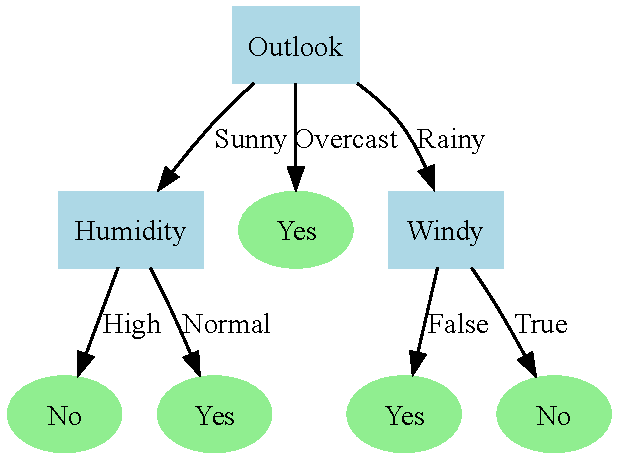
\includegraphics[width=0.9\textwidth]{id3_weather.pdf}
		\caption{Arbre ID3 simplifié sur le dataset météo.}
	\end{figure}
\end{frame}

\begin{frame}
	\frametitle{Dataset Drug200 : version complète vs réduite}
	\begin{itemize}
		\item Version complète : \texttt{Age}, \texttt{Sex}, \texttt{BP}, \texttt{Cholesterol}, \texttt{Na\_to\_K}, \texttt{Drug}.
		\item Pour ID3, on a supprimé les variables numériques (\texttt{Age}, \texttt{Na\_to\_K}).
		\item But : éviter une branche par valeur et rendre l'arbre lisible.
	\end{itemize}
	\begin{figure}
		\centering
		\scriptsize
		\begin{tabular}{@{} r c c c c c @{}}
			\toprule
			\textbf{Age} & \textbf{Sex} & \textbf{BP} & \textbf{Chol} & \textbf{Na\_to\_K} & \textbf{Drug} \\
			\midrule
			23 & F & HIGH & HIGH & 25.355 & drugY \\
			47 & M & LOW  & HIGH & 13.093 & drugC \\
			47 & M & LOW  & HIGH & 10.114 & drugC \\
			28 & F & NORMAL & HIGH & 7.798 & drugX \\
			61 & F & LOW & HIGH & 18.043 & drugY \\
			\vdots & \vdots & \vdots & \vdots & \vdots & \vdots \\
			56 & F & LOW & HIGH & 11.567 & drugC \\
			16 & M & LOW & HIGH & 12.006 & drugC \\
			52 & M & NORMAL & NORMAL & 9.894 & drugX \\
			23 & M & NORMAL & NORMAL & 14.020 & drugX \\
			40 & F & LOW & NORMAL & 11.349 & drugX \\
			\bottomrule
		\end{tabular}
		\caption{Extrait du dataset Drug200.}
	\end{figure}
\end{frame}

\begin{frame}
	\frametitle{ID3 sur Drug200 : problème des variables continues}
	\begin{itemize}
		\item Avec \texttt{.unique()}, une valeur numérique $\Rightarrow$ une branche.
		\item Résultat : arbre très large et peu interprétable.
	\end{itemize}
	\begin{figure}
		\centering
		
\includegraphics[width=0.9\textwidth]{id3_limitations.pdf}
		\caption{Exemple d'explosion de branches avec des variables continues.}
	\end{figure}
\end{frame}

\begin{frame}
	\frametitle{Zoom sur une zone de l'arbre}
	\begin{figure}
		\centering
		\vspace{-1.8em}
		\hspace*{-10\textwidth}
		
\includegraphics[width=20\textwidth,clip]{id3_limitations.pdf}
		\caption{Zoom pour rendre la structure lisible.}
	\end{figure}
\end{frame}

\begin{frame}
	\frametitle{ID3 sur Drug200 (variables catégorielles)}
	\begin{figure}
		\centering
		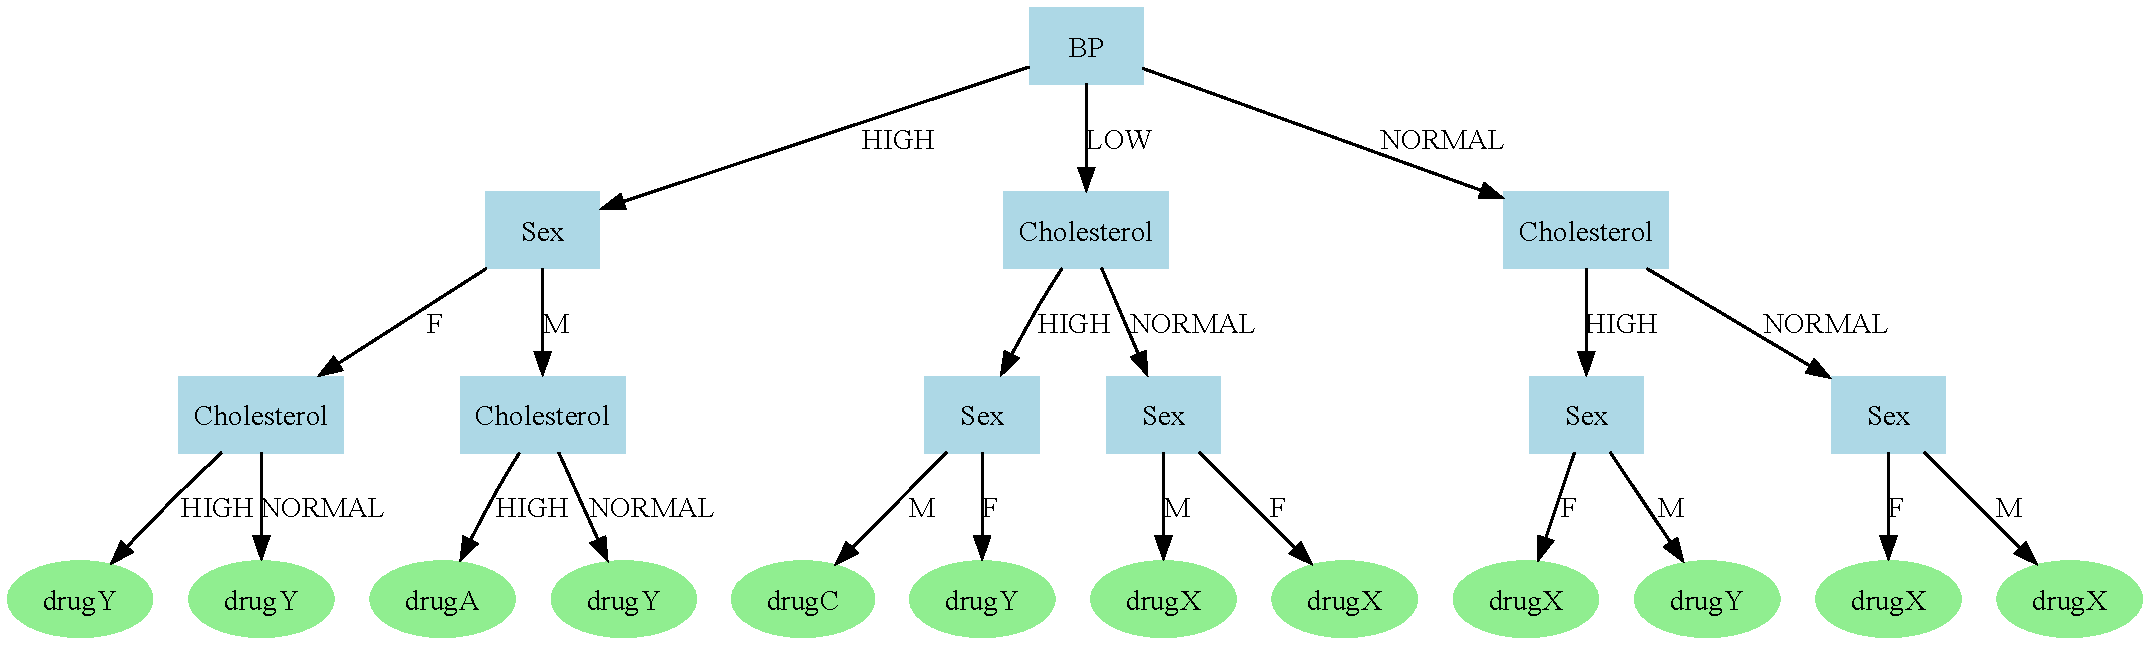
\includegraphics[width=0.9\textwidth]{id3_drug200_cat.pdf}
		\caption{Exemple d'arbre ID3 sur Drug200 sans variables continues.}
	\end{figure}
\end{frame}

\begin{frame}
	\frametitle{Pourquoi CART corrige ce problème}
	\begin{itemize}
		\item CART gère les variables numériques en testant des seuils.
		\item Chaque split est binaire ($\le t$ / $> t$), donc pas d'explosion de branches.
		\item Résultat : un arbre plus lisible et plus stable.
	\end{itemize}
\end{frame}

\subsection{Classification and Regression Trees (CART)}
\begin{frame}
	\frametitle{Classification and Regression Trees (CART)}
	\begin{algorithm}[H]
	\scriptsize
    \caption{Algorithme CART}
    \begin{algorithmic}[1]
        \Procedure{CART}{$D$}
            \If{critère d'arrêt atteint (pureté, profondeur max, etc.)}
                \State \Return nœud feuille avec la classe majoritaire
            \EndIf

            \State \textbf{Recherche de la séparation optimale :}
            \State $(j, t) \gets \text{Trouver l'attribut } j \text{ et le seuil } t \text{ minimisant l'indice de \textbf{Gini}}$

            \State \textbf{Division binaire :}
            \State $D_{gauche} \gets \{x \in D \mid x_j \le t\}$
            \State $D_{droite} \gets \{x \in D \mid x_j > t\}$

            \State Créer un nœud $Racine$ divisé par le test $(x_j \le t)$
            \State $Racine.gauche \gets$ \Call{CART}{$D_{gauche}$}
            \State $Racine.droite \gets$ \Call{CART}{$D_{droite}$}

            \State \Return $Racine$
        \EndProcedure
    \end{algorithmic}
    \end{algorithm}
\end{frame}

\begin{frame}
	\frametitle{CART sur l'exemple météo (Quinlan 1989)}
	\begin{figure}
		\centering
		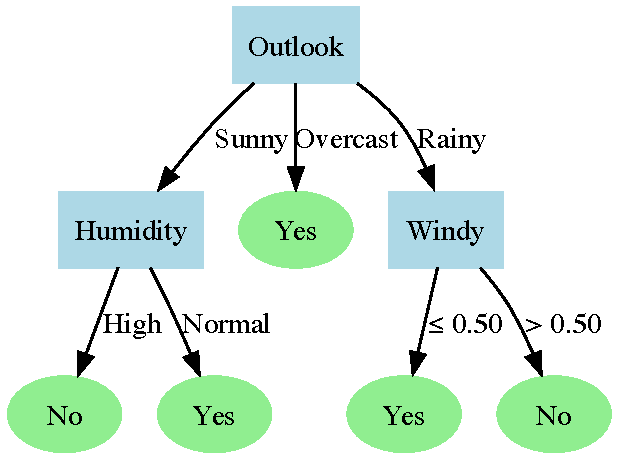
\includegraphics[width=0.9\textwidth]{cart_weather.pdf}
		\caption{Exemple de CART sur le dataset météo.}
	\end{figure}
\end{frame}

\begin{frame}
	\frametitle{CART sur Drug200}
	\begin{figure}
		\centering
		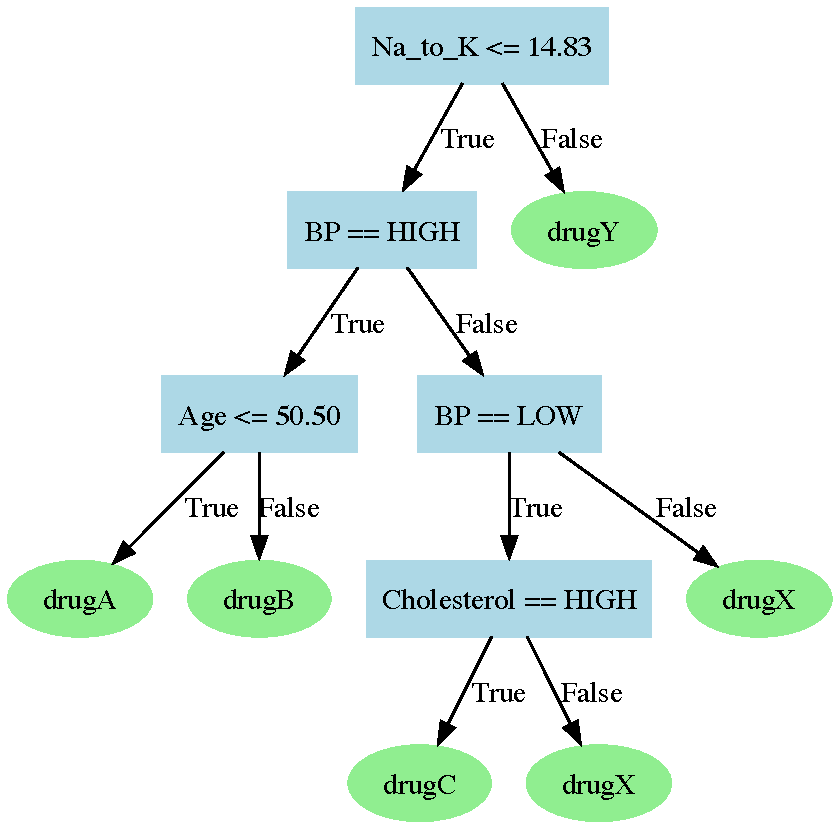
\includegraphics[width=\textwidth,height=0.7\textheight,keepaspectratio]{cart_drug200.pdf}
		\caption{Exemple de CART sur le dataset Drug200.}
	\end{figure}
\end{frame}

\begin{frame}
	\frametitle{Dataset Breast Cancer : aperçu}
	\begin{figure}
		\centering
		\scriptsize
		\begin{tabular}{@{} r c c c c c c c @{}}
			\toprule
			\textbf{Age} & \textbf{Race} & \textbf{T} & \textbf{N} & \textbf{Grade} & \textbf{Tumor} & \textbf{Nodes+} & \textbf{Status} \\
			\midrule
			68 & White & T1 & N1 & 3 & 4  & 1 & Alive \\
			50 & White & T2 & N2 & 2 & 35 & 5 & Alive \\
			58 & White & T3 & N3 & 2 & 63 & 7 & Alive \\
			58 & White & T1 & N1 & 3 & 18 & 1 & Alive \\
			47 & White & T2 & N1 & 3 & 41 & 1 & Alive \\
			\vdots & \vdots & \vdots & \vdots & \vdots & \vdots & \vdots & \vdots \\
			62 & Other & T1 & N1 & 2 & 9  & 1 & Alive \\
			56 & White & T2 & N2 & 2 & 46 & 8 & Alive \\
			68 & White & T2 & N1 & 2 & 22 & 3 & Alive \\
			58 & Black & T2 & N1 & 2 & 44 & 1 & Alive \\
			46 & White & T2 & N1 & 2 & 30 & 2 & Alive \\
			\bottomrule
		\end{tabular}
		\caption{Extrait du dataset Breast Cancer.}
	\end{figure}
\end{frame}

\begin{frame}
	\frametitle{CART sur Breast Cancer}
	\begin{figure}
		\centering
		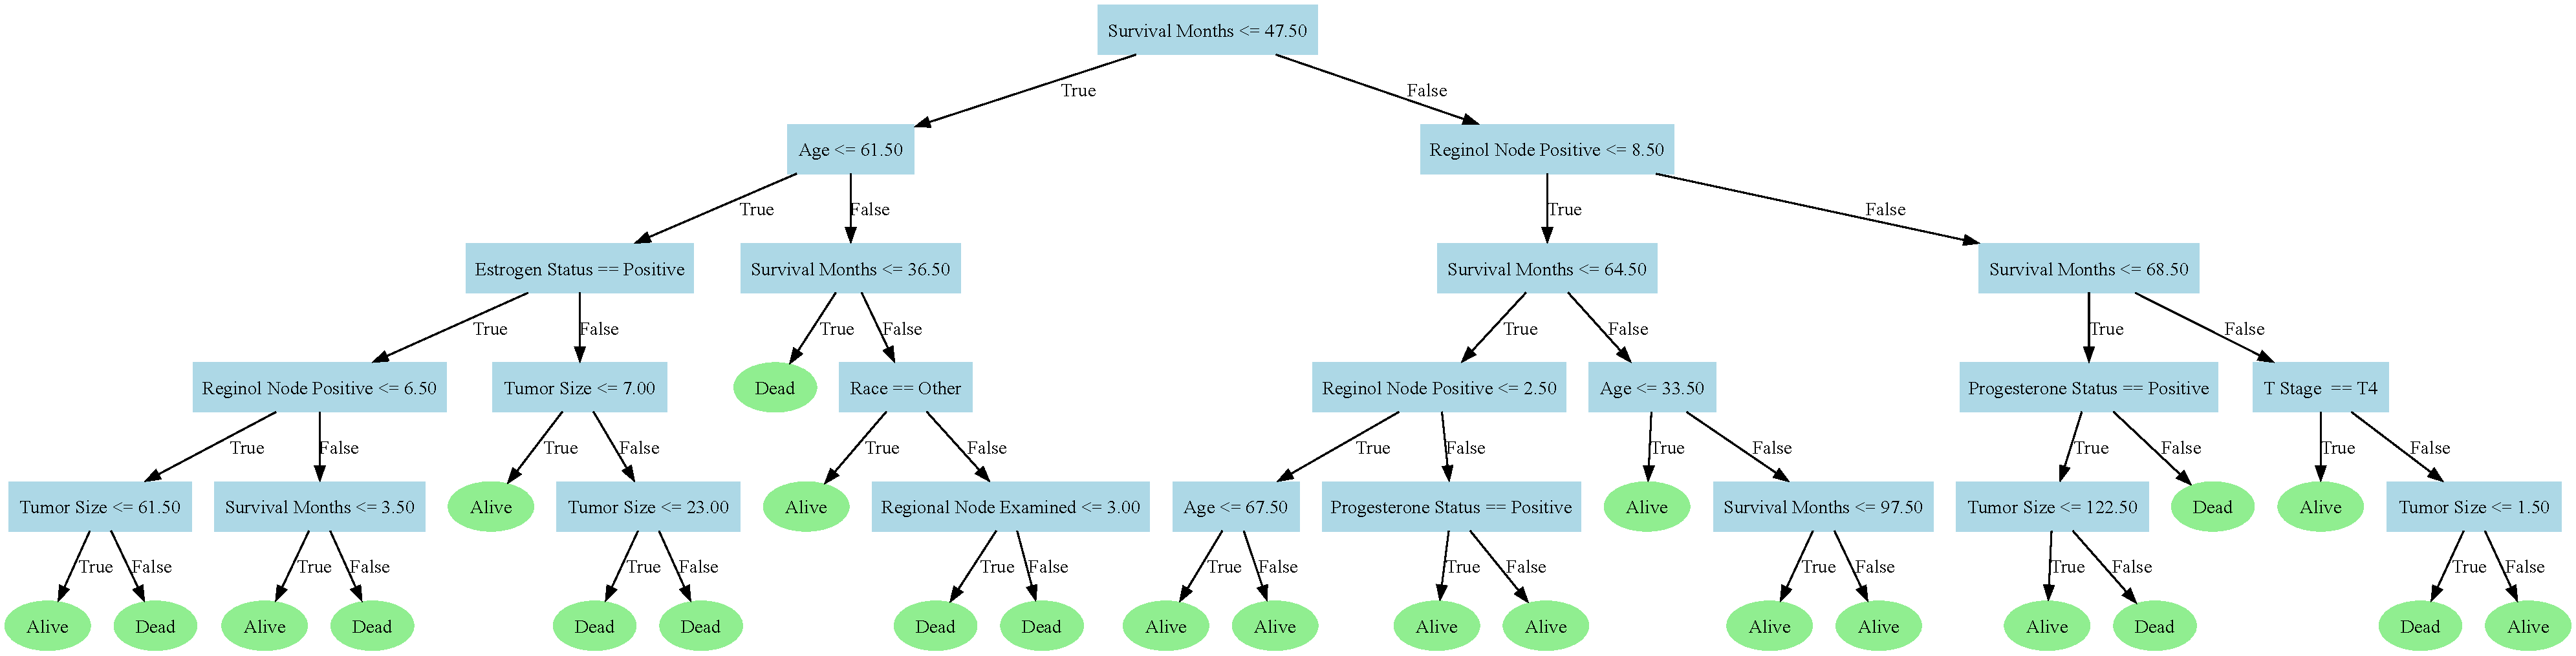
\includegraphics[width=\textwidth,height=0.72\textheight,keepaspectratio]{cart_breast_cancer.pdf}
		\caption{Exemple de CART sur un dataset médical.}
	\end{figure}
\end{frame}

\begin{frame}
    \frametitle{ID3 vs CART : Synthèse}
    \begin{table}
        \renewcommand{\arraystretch}{1.2}
        \begin{tabular}{@{} lll @{}}
            \toprule
            \textbf{Caractéristique} & \textbf{ID3} & \textbf{CART} \\
            \midrule
            Critère & Entropie & Gini \\
            Type d'arbre & Multi-branches & Binaire uniquement \\
            Tâches & Classification & Classif. \& Régression \\
            Élagage & Non & Oui (Pruning) \\
            \bottomrule
        \end{tabular}
    \end{table}
\end{frame}

\section{Élagage d'arbre}

\begin{frame}
	\frametitle{Pourquoi élaguer ?}
	\begin{itemize}
		\item Un arbre trop profond mémorise les données d'entraînement.
		\item En test, il généralise moins bien : c'est le surapprentissage.
		\item L'élagage enlève des branches peu utiles pour rendre l'arbre plus simple.
	\end{itemize}
\end{frame}

\begin{frame}
	\frametitle{Post-pruning (CART)}
	\begin{itemize}
		\item Étape 1 : entraîner un arbre complet (très détaillé).
		\item Étape 2 : couper une branche candidate.
		\item Étape 3 : tester la précision sur un jeu de validation.
		\item Étape 4 : si la précision ne baisse pas, on garde la version simplifiée.
		\item On répète : moins de branches inutiles $\Rightarrow$ meilleure généralisation.
	\end{itemize}
	\vspace{0.4em}
	\footnotesize
\end{frame}

\begin{frame}
	\frametitle{Pseudocode : élagage (post-pruning)}
	\scriptsize
	\textbf{Notations :} $T$ = arbre courant,\; $D_{val}$ = données de validation,\; $T'$ = arbre simplifié.\\
	\vspace{0.3em}
	\begin{algorithm}[H]
	\caption{Post-pruning (version simple)}
	\begin{algorithmic}[1]
		\Procedure{Prune}{$T, D_{val}$}
			\For{chaque nœud interne $n$ (du bas vers le haut)}
				\State $T' \gets$ arbre où $n$ devient une feuille
				\If{accuracy($T'$, $D_{val}$) $\ge$ accuracy($T$, $D_{val}$)}
					\State $T \gets T'$
				\EndIf
			\EndFor
			\State \Return $T$
		\EndProcedure
	\end{algorithmic}
	\end{algorithm}
\end{frame}

\begin{frame}
	\frametitle{Résultats élagage (placeholder)}
	\begin{figure}
		\centering
		\fbox{\parbox[c][3.8cm][c]{0.85\textwidth}{\centering Placeholder : précision train/val avant/après pruning}}
		\caption{Impact de l'élagage sur la performance.}
	\end{figure}
\end{frame}

\section{Random Forest}

\begin{frame}
	\frametitle{Idée générale}
	\begin{itemize}
		\item On entraîne plusieurs arbres différents.
		\item Chaque arbre voit un échantillon aléatoire des données (bootstrap).
		\item Chaque nœud teste un petit sous-ensemble de features.
		\item On combine les prédictions : vote majoritaire ou moyenne.
	\end{itemize}
\end{frame}

\begin{frame}
	\frametitle{Schéma d'ensemble}
	\begin{figure}
		\centering
		\fbox{\parbox[c][4.0cm][c]{0.85\textwidth}{\centering Placeholder : schéma Random Forest}}
	\end{figure}
\end{frame}

\begin{frame}
	\frametitle{Paramètres usuels}
	\begin{itemize}
		\item Nombre d'arbres $n\_{trees}$.
		\item Profondeur max / taille minimale des feuilles.
		\item Sous-ensemble de features : $p=\sqrt{d}$ en classification.
	\end{itemize}
\end{frame}

\begin{frame}
	\frametitle{Pseudocode : Random Forest}
	\scriptsize
	\begin{algorithm}[H]
	\caption{Random Forest (classification)}
	\begin{algorithmic}[1]
		\Procedure{RF}{$D, n\_{trees}$}
			\For{$i=1$ à $n\_{trees}$}
				\State $D_i \gets$ bootstrap($D$)
				\State $T_i \gets$ \Call{CART}{$D_i$} avec sous-ensemble aléatoire de features à chaque nœud
			\EndFor
			\State \Return $\{T_1,\dots,T_{n\_{trees}}\}$
		\EndProcedure
		\Statex
		\Procedure{Predict}{$\{T_i\}, x$}
			\State prédictions $\gets \{T_i(x)\}$
			\State \Return vote\_majoritaire(prédictions)
		\EndProcedure
	\end{algorithmic}
	\end{algorithm}
\end{frame}

\begin{frame}
	\frametitle{Résultats Random Forest (placeholder)}
	\begin{figure}
		\centering
		\fbox{\parbox[c][3.8cm][c]{0.85\textwidth}{\centering Placeholder : accuracy/erreur RF vs arbre seul}}
		\caption{Comparaison Random Forest vs arbre unique.}
	\end{figure}
\end{frame}

\section{Limites et conclusion}

\begin{frame}
	\frametitle{Limites}
	\begin{itemize}
		\item Sensible au bruit et aux petites variations des données.
		\item Biais vers des attributs à nombreuses valeurs (ID3).
		\item Solutions : élagage, critères pénalisés, ensembles (Random Forest).
	\end{itemize}
\end{frame}

\begin{frame}
	\frametitle{Conclusion}
	\begin{itemize}
		\item Les arbres : interprétables et efficaces.
		\item ID3 : simple, entropie, multi-branches.
		\item CART : binaire, Gini, gère les variables continues + pruning.
		\item Perspectives : ensembles pour améliorer la robustesse.
	\end{itemize}
\end{frame}

\end{document}
